\documentclass{article}

\usepackage{booktabs}
\usepackage[margin=1in]{geometry}
\usepackage{makecell}
\usepackage[version=4]{mhchem}
\usepackage{microtype}
\usepackage{siunitx}
\DeclareSIUnit\wavenumber{\per\centi\metre}
\usepackage{threeparttable}

\begin{document}
Harmonic frequencies of CO2 anharmonic stretch across different ionic liquids - effects of BSSE and CP

\section{Summary}

\begin{table}
  \centering
  \caption{CP correction turned on?}
  \begin{tabular}{ccc}
    \toprule
    geom & freq & {\(R^2\) with uncorrected frequency trends} \\
    \midrule
    N & N & 1.000 \\
    N & Y & 0.440 \\
    Y & N & \textbf{0.888} \\
    Y & Y & \textbf{0.629} \\
    \bottomrule
  \end{tabular}
\end{table}

\begin{table}
  \centering
  \caption{ALMO turned on?}
  \begin{tabular}{ccc}
    \toprule
    geom & freq & {\(R^2\) with uncorrected frequency trends} \\
    \midrule
    N & N & 1.000 \\
    N & Y & 0.011 \\
    Y & N & \textbf{0.978} \\
    Y & Y & 0.197 \\
    \bottomrule
  \end{tabular}
\end{table}

\section{CP geometries}

This table is already in the SI

\begin{table}
  \centering
  \caption{Frequencies are not with CP-corrected Hessians. Q-Chem, B3LYP/6-31G**, (100,302) to reproduce 1st paper. 2nd column is results from 1st paper. Positive diff is redshift. All values have units of \si{\wavenumber}.}
  \begin{tabular}{cSSS}
    \toprule
    Anion & \text{CP geom frequency} & \text{no CP geom frequency} & \text{Diff [without – with]} \\
    \midrule
    \ce{[TFA]-} & 2428.05 & 2429.31 & 1.26 \\
    \ce{[SCN]^-_S} & 2427.91 & 2430.24 & 2.33 \\
    \ce{[DCA]-} & 2426.6 & 2430.47 & 3.87 \\
    \ce{[SCN]^-_N} & 2427.95 & 2431.64 & 3.69 \\
    \ce{[TfO]-} & 2428.95 & 2431.91 & 2.96 \\
    \ce{[BF4]-} & 2431.48 & 2434.69 & 3.21 \\
    \ce{[Tf2N]-} & 2431.49 & 2435.8 & 4.31 \\
    \ce{[PF6]-} & 2432.58 & 2437.74 & 5.16 \\
    \bottomrule
  \end{tabular}
\end{table}

This table is already in the SI

\begin{table}
  \centering
  \caption{CP geom?/CP freq?}
  \begin{tabular}{cSSSS}
    \toprule
    Anion & \text{no/no} & \text{yes/no} & \text{no/yes} & \text{yes/yes} \\
    \midrule
    \ce{[TFA]-} & 2429.31 & 2428.05 & 2457.238 & 2440.879 \\
    \ce{[SCN]^-_S} & 2430.24 & 2427.91 & 2445.642 & 2438.003 \\
    \ce{[DCA]-} & 2430.47 & 2426.60 & 2436.113 & 2431.383 \\
    \ce{[SCN]^-_N} & 2431.64 & 2427.95 & 2432.691 & 2437.876 \\
    \ce{[TfO]-} & 2431.91 & 2428.95 & 2441.921 & 2443.665 \\
    \ce{[BF4]-} & 2434.69 & 2431.48 & 2454.767 & 2450.890 \\
    \ce{[Tf2N]-} & 2435.80 & 2431.49 & 2451.851 & 2441.309 \\
    \ce{[PF6]-} & 2437.74 & 2432.58 & 2479.806 & 2469.473 \\
    \bottomrule
  \end{tabular}
\end{table}

\begin{figure}
  \centering
  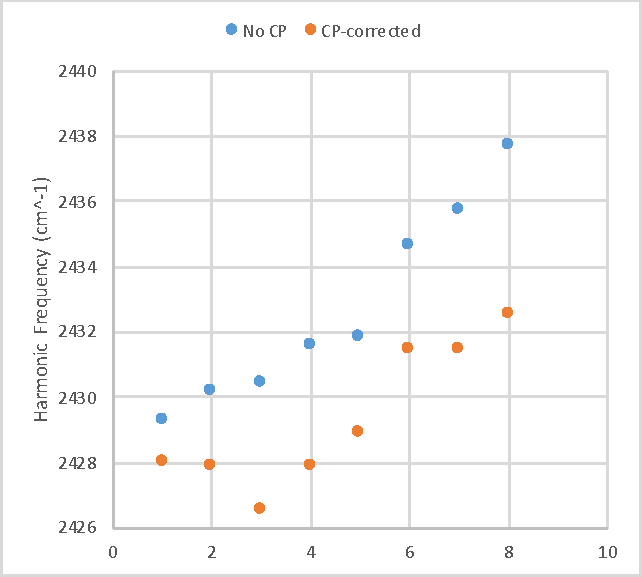
\includegraphics{./002_2_1.pdf}
\end{figure}

\begin{figure}
  \centering
  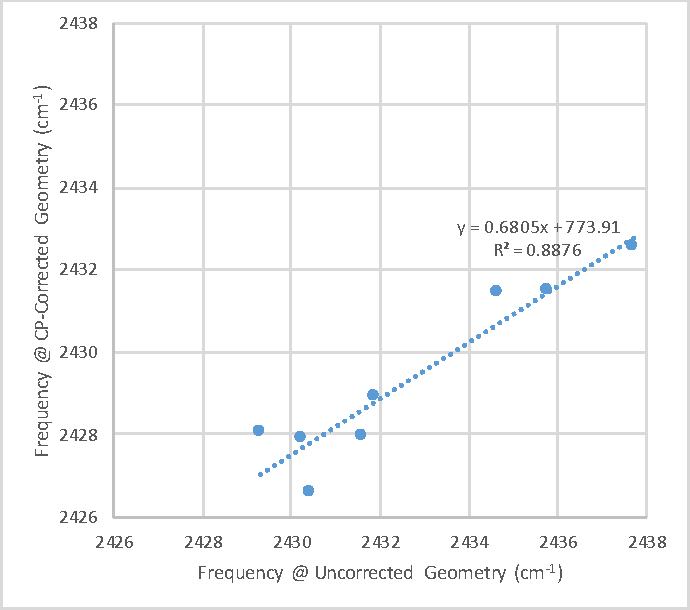
\includegraphics{./002_2_2.pdf}
\end{figure}

\begin{figure}
  \centering
  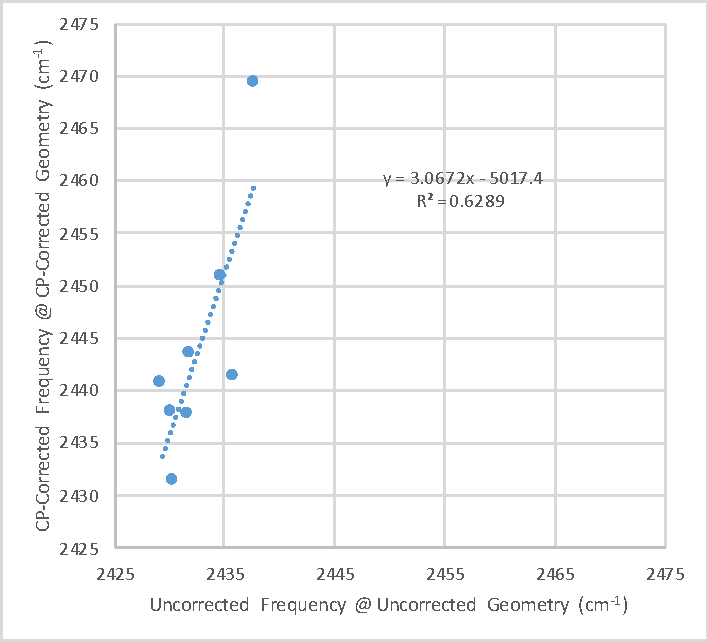
\includegraphics{./002_2_3.pdf}
\end{figure}

\begin{figure}
  \centering
  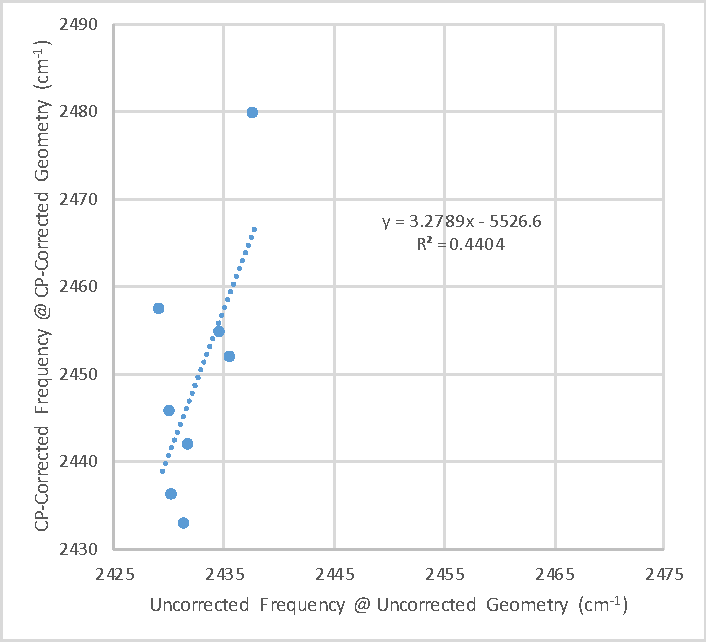
\includegraphics{./002_2_4.pdf}
\end{figure}

\begin{figure}
  \centering
  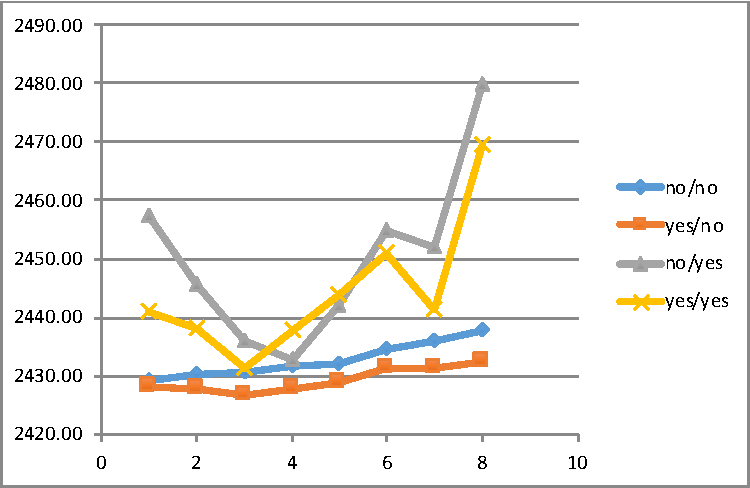
\includegraphics{./002_2_5.pdf}
\end{figure}

\section{ALMO}

\begin{table}
  \centering
  \begin{tabular}{cSSSS}
    \toprule
    Anion & {full} & {\makecell{ALMO geom \\ SCF Hessian}} & {\makecell{ALMO geom \\ ALMO Hessian}} & {\makecell{SCF geom \\ ALMO Hessian}} \\
    \midrule
    \ce{[BF4]-} & 2434.70 & 2438.56 & 2441.62 & 2437.69 \\
    \ce{[DCA]-} & 2430.90 & 2439.10 & 2442.59 & 2434.75 \\
    \ce{[PF6]-} & 2437.50 & 2438.47 & 2441.03 & 2440.03 \\
    \ce{[SCN]-} & 2430.30 & 2438.78 & 2441.37 & 2433.14 \\
    \ce{[TFA]-} & 2429.80 & 2438.39 & 2441.06 & 2432.93 \\
    \ce{[Tf2N]-} & 2437.70 & 2438.76 & 2440.85 & 2439.46 \\
    \ce{[TfO]-} & 2433.90 & 2439.37 & 2442.54 & 2436.75 \\
    \bottomrule
  \end{tabular}
\end{table}

TODO 2 figures?

\section{Detailed \ce{BF4}}

\begin{table}
  \centering
  \caption{\ce{[C1C1im][BF4]}. All calculations use B3LYP/6-31G**. The CP geometry is from Cuby driving Turbomole. The no CP geometry is from Q-Chem. (100,302) is the grid used in all calculations for the 1st paper.}
  \begin{threeparttable}
    \begin{tabular}{ccccS}
      \toprule
      Geometry? & Hessian? & Program & XC grid & {Frequency (\si{\wavenumber})} \\
      \midrule
      CP & CP & Cuby (Turbomole) & 7 & 2450.89 \\
      CP & CP & Cuby (Turbomole) & m5 & 2450.871 \\
      CP & no CP & Cuby (Turbomole) & 7 & 2435.634 \\
      CP & no CP & Turbomole & 7 & 2434.72\tnote{1} \\
      CP & no CP & Q-Chem & (75,302) & 2431.55 \\
      CP & no CP & Q-Chem & (100,302) & 2431.48\tnote{2} \\
      CP & no CP & Q-Chem & (99,590) & 2431.77\tnote{3} \\
      no CP & no CP & Q-Chem & (100,302) & 2434.69 \\
      no CP & CP & Cuby (Turbomole) & 7 & 2454.767 \\
      \bottomrule
    \end{tabular}
    \begin{tablenotes}
    \item[1] Difference Hessian no CP/CP: \(2450.89 - 2434.72 = 16.17\)
    \item[2] \((100,302) - (75,302) = -0.07\)
    \item[3] \((99,590) - (75,302) = 0.22\)
    \end{tablenotes}
  \end{threeparttable}
\end{table}

\section{Detailed \ce{PF6}}

\begin{table}
  \centering
  \caption{\ce{[C1C1im][PF6]}. All calculations use B3LYP/6-31G**. The CP geometry is from Cuby driving Turbomole. The no CP geometry is from Q-Chem. (100,302) is the grid used in all calculations for the 1st paper.}
  \begin{threeparttable}
    \begin{tabular}{ccccS}
      \toprule
      Geometry? & Hessian? & Program & XC grid & {Frequency (\si{\wavenumber})} \\
      \midrule
      CP & CP & Cuby (Turbomole) & 7 & 2469.473 \\
      CP & no CP & Cuby (Turbomole) & 7 & 2436.846 \\
      CP & no CP & Turbomole & 7 & 2435.93\tnote{1} \\
      CP & no CP & Q-Chem & (75,302) & 2432.81 \\
      CP & no CP & Q-Chem & (100,302) & 2432.58\tnote{2} \\
      CP & no CP & Q-Chem & (99,590) & 2432.99\tnote{3} \\
      no CP & no CP & Q-Chem & (100,302) & 2437.74 \\
      no CP & CP & Cuby (Turbomole) & 7 & 2479.806 \\
      \bottomrule
    \end{tabular}
    \begin{tablenotes}
    \item[1] Difference Hessian no CP/CP: \(2469.473 - 2435.93 = 33.543\)
    \item[2] \((100,302) - (75,302) = -0.23\)
    \item[3] \((99,590) - (75,302) = 0.18\)
    \end{tablenotes}
  \end{threeparttable}
\end{table}

\end{document}
